%-----------------------------------------------------
% Chapter: Prototype Implementation
%-----------------------------------------------------
\chapter{Implementation}
\label{chap:implementation}
\section{Hardware Specification}
All implementation was completed on a personal machine. The hardware specifications for the machine are highlighted below

\begin{table}[h!]
	\centering
	\begin{tabular}{||c | c||} 
		\hline
		Hardware Component & Specification \\ [0.5ex] 
		\hline\hline
		CPU & Intel Core i7-8750H CPU @ 2.20GHz x 12 \\ 
		GPU & NVIDIA GeForce GTX 1050 Ti 4GB \\
		RAM & 16GB \\
		4 & 545 \\ [1ex] 
		\hline
	\end{tabular}
	\caption{Hardware specification for machine used throughout development}
	\label{table:1}
\end{table}
\section{Calculating Co-occurrence Statistics}
Many unsupervised natural language processing methods compute co-occurrence statistics before learning takes place. Typical co-occurrence statistics, such as GloVe's word-word co-occurrence matrix are very sparse in nature, and computing them can often be a computationally more expensive task than the learning itself. Examining GloVe, where a corpus has vocabulary size \(N\), a word-word co-occurrence matrix \(X\) is computed with \(X_{ij}\) being a measure of the number of times words \(i\) and \(j\) co-occur within a given context window. 

\noindent
\newline
The original GloVe paper describes this process as a \textit{'one-time upfront cost'}, with the assumption that selected corpora are static. Unfortunately, for many natural language processing pipelines such corpora are more dynamic in nature. For example, social data from online platforms such as Twitter are in constant flux and relying on pre-computed co-occurrence statistics is sub-optimal. Compared to GloVe, computing the co-occurrence statistics for CoVeR has added complexity due to the transition from a co-occurrence matrix to a co-occurrence tensor. 

\noindent
\newline
Methods for efficient computation of co-occurrence statistics include the usage of distributed computing techniques such as \textit{MapReduce}. MapReduce is a model for distributed computing which involves two functional processes namely map and reduce. During the \textit{map} process, data is taken in as key/value pairs and transformed to intermediary key/value pairs as output. These are then passed to the \textit{reduce} process which aggregates data which share the same key.

\noindent
\newline
Apache Spark is an open-source framework, written in Scala, for distributed computing and has recently emerged as the preferred option for big data processing over Apache Hadoop. Like Hadoop, Spark also supports the MapReduce programming paradigm but boasts features such as enhanced speed, a distributed data structure, as well as API's written in multiple programming languages. Spark uses a master/slave architecture to achieve distributed computing. The \textit{driver} acts as the master node and distributes tasks to many different worker nodes, also known as \textit{executors}, which each run their own JVM processes to execute tasks.

\begin{figure}[h]
	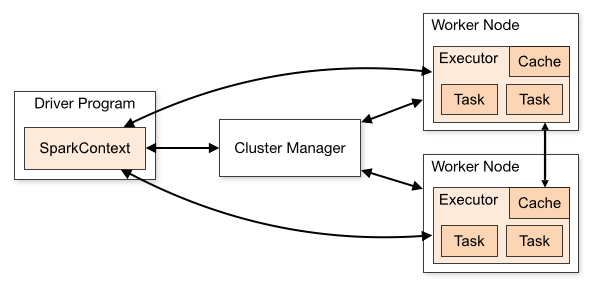
\includegraphics[width=12cm, height=6cm]{./figures/fig5}
	\centering
	\caption{High level view of the Spark Architecture. The spark context is where the main program is defined, which is then split into tasks to be completed via numerous executors.}
	\label{fig:fig5}
\end{figure}

\noindent
\newline
PySpark, a Python API for the Spark framework was initially used to both pre-process data and calculate co-occurrence statistics for the corpora. 
Unfortunately, the overhead of collecting completed executor tasks to the driver as well as the  cross language communication between Python and Scala made PySpark an unfavourable option for collecting co-occurrence statistics. A similar parallelised approach which avoided cross language communication involved the use of Python's multiprocessing module. This  approach suffered from the restrictions of Pythons Global Interpreter Lock (GIL) which prevents shared access of Python objects across multiple threads. 

\noindent
\newline
Cython is a superset of the Python programming language which aims to provide C like performance whilst maintaining the ability to write Python like code. Native Python programs can experience major speed improvements using Cython because of its ability to compile Python to C code. 

\section{CoVeR Implementation}
At time of writing, no publicly available implementation of CoVeR is available. As a result and to meet the needs of this project, CoVeR was implemented from scratch using the PyTorch library. PyTorch is a Python library based on Torch, which supports Numpy like operations which can be accelerated through the GPU. All supporting code for the implementation can be found here: (LINK TO CODE)
\subsection{Initialisation of Learnable Parameters} 
\subsection{Hyperparameters}

\section{Model Implementation}
Implementation of both the language model and the text classifier was done using Keras. Keras is a high level machine learning library written in Python, which runs on top of either Tensorflow or Theano. The motivation behind using Keras comes from its ease of use to quickly develop deep learning networks. In this project Keras is deployed using Tensorflow as a backend, specifically for its GPU capabilities.
\subsection{Language Model}
The structure for the language model can be seen in Figure X.X. The model consisted of an input layer, an embedding layer, a bidirectional LSTM, a dropout layer and finally a dense layer.
\subsubsection{Hyperparameter Tuning}
\subsection{Text Classifier}
\subsubsection{Hyperparameter Tuning}
\section{SONGIFAI}
\subsection{Architecture}
\subsubsection{Client Side}
For the client-side development of SONGIFGAI, a main requirement refers to the systems availability for web and mobile access. Being a prototype solution, it was important that the development was swift and well structured so that the research goals of the project were not hindered. To help achieve this, ReactJS was chosen as the front-end development framework.

\noindent
\newline
React is a Javascript framework for building user interfaces originally developed and maintained by Facebook. The main advantages of using React
\subsubsection{Server Side}
Requirements ... refer to a user of the system being able to save, load and edit their lyrics. Moreover for easy compatibility with the Keras generated models, another Python based library was preferred as the for the server side. To meet these conditions, Django was chosen as the development framework for the back-end of the system. Django is a python based web framework which follows the model-view-template (MVT) architectural pattern.
\subsection{Class Overview}